\chapter{Naive Bayes}

\section{Pré-traitement des données}

Nous avons d'abord effectué un pré-traitement des données en utilisant différentes techniques :

\subsection{Tokenisation des commentaires}

Nous avons utilisé la tokenisation pour diviser les commentaires en tokens individuels.

\subsubsection*{Tokenisation à l'aide de nôtre API \texttt{tokenize\_apy}}

La tokenisation des commentaires a été réalisée en utilisant l'API \texttt{tokenize\_apy}.

\subsubsection*{Équilibrage du jeu de données}

Nous avons équilibré le jeu de données en échantillonnant un nombre égal de commentaires toxiques et non toxiques.

\section{Analyse exploratoire des données}

Voici les statistiques descriptives sur le jeu de données équilibré :

\subsection{Statistiques descriptives}

\begin{itemize}
    \item Nombre total de documents : 25 962
    \item Nombre total de tokens : 127 656
    \item Nombre de classes à prédire : 2 (toxique ou non toxique)
    \item Les tokens les plus fréquents incluent "grand", "ter", "burn", etc.
\end{itemize}

\section{Entraînement du modèle}

Nous avons entraîné le modèle Bayésien naïf en suivant les étapes suivantes :

\subsection{Préparation des données}

\begin{itemize}
    \item Calcul de la fréquence des mots et sélection des stop words.
    \item Entraînement du modèle en utilisant \texttt{CountVectorizer} et \texttt{MultinomialNB}.
\end{itemize}

\subsection{Évaluation des performances du modèle}

Les "Feature Dimensions" indiquent la taille de la matrice de caractéristiques utilisée pour chaque méthode. Le premier nombre représente le nombre d'échantillons (lignes) dans l'ensemble de données, et le deuxième nombre représente le nombre de caractéristiques (colonnes) générées par le vectoriseur.
\begin{table}[htbp]
    \centering
    \caption{Combined Classification Reports Across Different Methods}
    \resizebox{\textwidth}{!}{%
    \begin{tabular}{@{}lccccccccc@{}}
    \toprule
    \textbf{Method} & \textbf{Features Dimension} & \multicolumn{2}{c}{\textbf{Class 0}} & \multicolumn{2}{c}{\textbf{Class 1}} & \textbf{Accuracy} & \textbf{Macro Avg} & \textbf{Weighted Avg} \\
    & & \textbf{Precision} & \textbf{Recall} & \textbf{Precision} & \textbf{Recall} & & & \\
    \midrule
    comment\_text\_baseline & (127656, 165785) & 0.96 & 0.94 & 0.54 & 0.68 & 0.91 & (0.75, 0.81, 0.78) & (0.92, 0.91, 0.92) \\
    comment\_text\_bpe\_tokenize\_full\_normalization & (127656, 29611) & 0.97 & 0.93 & 0.53 & 0.77 & 0.91 & (0.75, 0.85, 0.79) & (0.93, 0.91, 0.92) \\
    comment\_text\_word\_tokenize\_no\_normalization & (127656, 165757) & 0.96 & 0.94 & 0.54 & 0.68 & 0.91 & (0.75, 0.81, 0.78) & (0.92, 0.91, 0.92) \\
    comment\_text\_gpt\_tokenize\_no\_normalization & (127656, 64839) & 0.96 & 0.93 & 0.50 & 0.64 & 0.90 & (0.73, 0.78, 0.75) & (0.91, 0.90, 0.91) \\
    comment\_text\_word\_tokenize\_normalization & (127656, 136809) & 0.97 & 0.94 & 0.56 & 0.69 & 0.92 & (0.76, 0.81, 0.78) & (0.93, 0.92, 0.92) \\
    comment\_text\_gpt\_tokenize\_normalization & (127656, 36098) & 0.97 & 0.92 & 0.49 & 0.69 & 0.90 & (0.73, 0.81, 0.76) & (0.92, 0.90, 0.91) \\
    comment\_text\_word\_tokenize\_full\_normalization & (127656, 134296) & 0.97 & 0.94 & 0.56 & 0.69 & 0.92 & (0.76, 0.81, 0.78) & (0.93, 0.92, 0.92) \\
    comment\_text\_gpt\_tokenize\_full\_normalization & (127656, 32705) & 0.97 & 0.93 & 0.52 & 0.73 & 0.91 & (0.74, 0.83, 0.78) & (0.93, 0.91, 0.91) \\
    comment\_text\_word\_tokenize\_simple\_normalization & (127656, 145452) & 0.97 & 0.94 & 0.54 & 0.69 & 0.91 & (0.75, 0.81, 0.78) & (0.92, 0.91, 0.92) \\
    comment\_text\_gpt\_tokenize\_simple\_normalization & (127656, 40563) & 0.97 & 0.91 & 0.48 & 0.74 & 0.90 & (0.73, 0.83, 0.76) & (0.92, 0.90, 0.91) \\
    comment\_text\_bpe\_tokenize\_simple\_dup\_normalization & (127656, 33322) & 0.97 & 0.92 & 0.51 & 0.77 & 0.90 & (0.74, 0.85, 0.78) & (0.93, 0.90, 0.91) \\
    comment\_text\_bpe\_tokenize\_no\_dup\_no\_punc\_normalization & (127656, 33402) & 0.97 & 0.92 & 0.51 & 0.77 & 0.91 & (0.74, 0.84, 0.78) & (0.93, 0.91, 0.91) \\
    \bottomrule
    \end{tabular}%
    }
\end{table}


\subsection{Validation croisée}

Nous avons également effectué une validation croisée en utilisant la métrique \texttt{f1\_macro}.

\begin{table}[h]
    \centering
    \begin{tabular}{|l|l|}
    \hline
    \textbf{Métrique} & \textbf{Score} \\ \hline
    f1\_macro (moyenne) & 0.8438 \\ \hline
    f1\_macro (écart type) & 0.0055 \\ \hline
    \end{tabular}
    \caption{Résultats de la validation croisée}
\end{table}

\section{Analyse des résultats}

\subsection{Calcul des probabilités}

\begin{itemize}
    \item Probabilités a priori pour chaque classe : \{0: 0.89831, 1: 0.10168\}
    \item Vocabulaire contient 33397 mots uniques
\end{itemize}

\subsection{Calcul des vraisemblances}

Nous avons calculé les probabilités conditionnelles (vraisemblances) pour chaque mot dans chaque classe.

\subsection{Prédiction}

Nous avons utilisé le modèle entraîné pour prédire la toxicité des commentaires de test. Par exemple, le commentaire "chretian attack" a été prédit comme toxique avec une probabilité de 0.000168.

\subsection{Matrice de confusion}

La matrice de confusion montre que le modèle prédit correctement les commentaires toxiques et non toxiques dans une large mesure.

\begin{figure}[h]
    \centering
    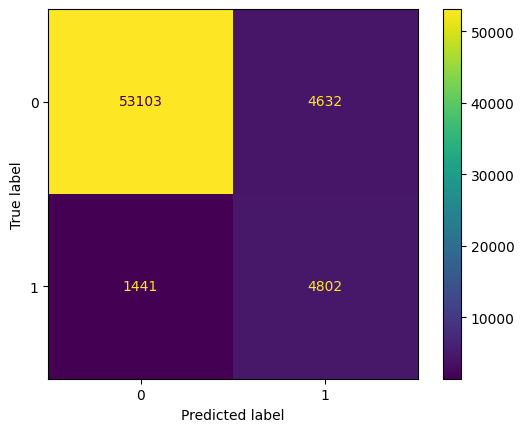
\includegraphics[width=.49\linewidth]{figures/matrix-confusion-naive_bayes.png}
    \caption{Matrice de confusion du modèle Bayésien naïf}
\end{figure}

\subsection{Etudes Annexe sur les données}
\begin{figure}[h]
        \centering
        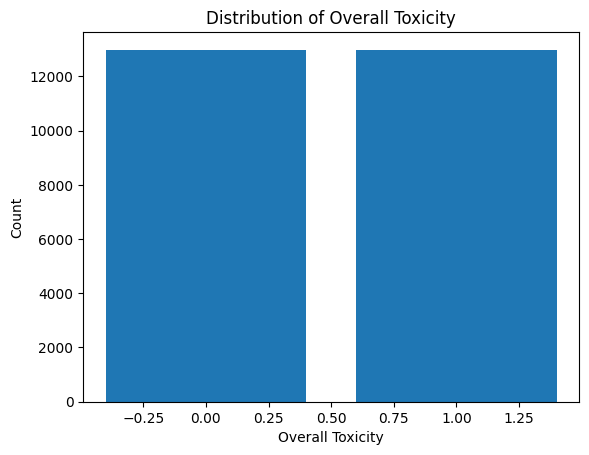
\includegraphics[width=.43\linewidth]{figures/distribution-toxicity-naive_bayes.png}
        \caption{Distribution de la toxicité des commentaires}
    \end{figure}

\begin{figure}[htbp]
    \centering
    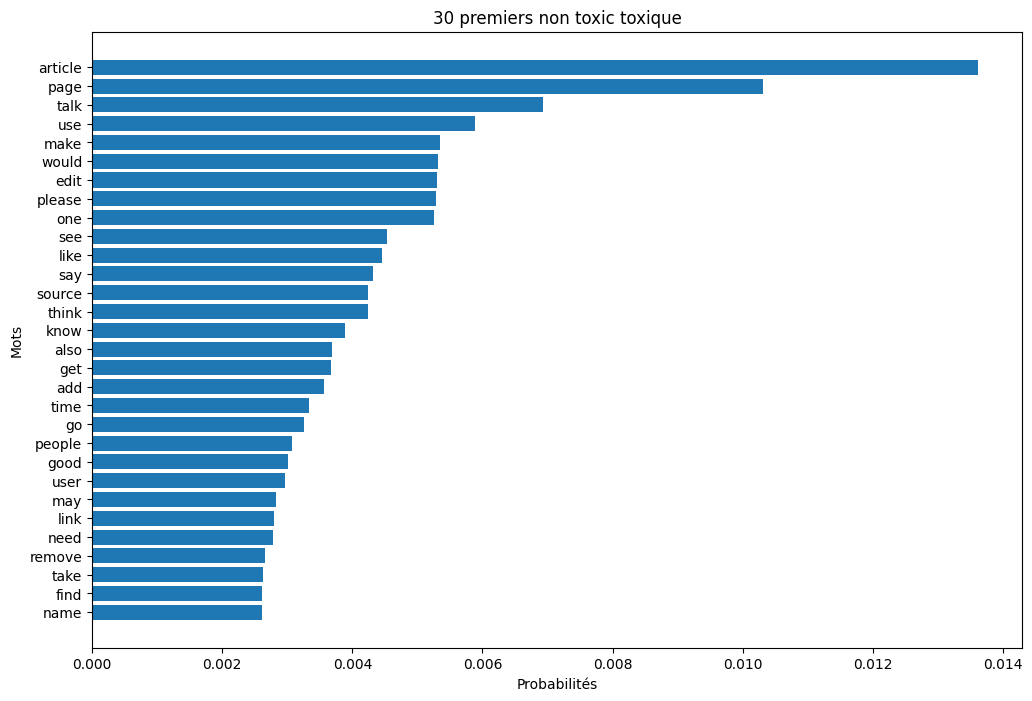
\includegraphics[width=.7\linewidth]{figures/30_first_non_toxic-naive_bayes.png}
    \caption{Top 30 mots non toxiques}
\end{figure}

\begin{figure}[htbp]
    \centering
    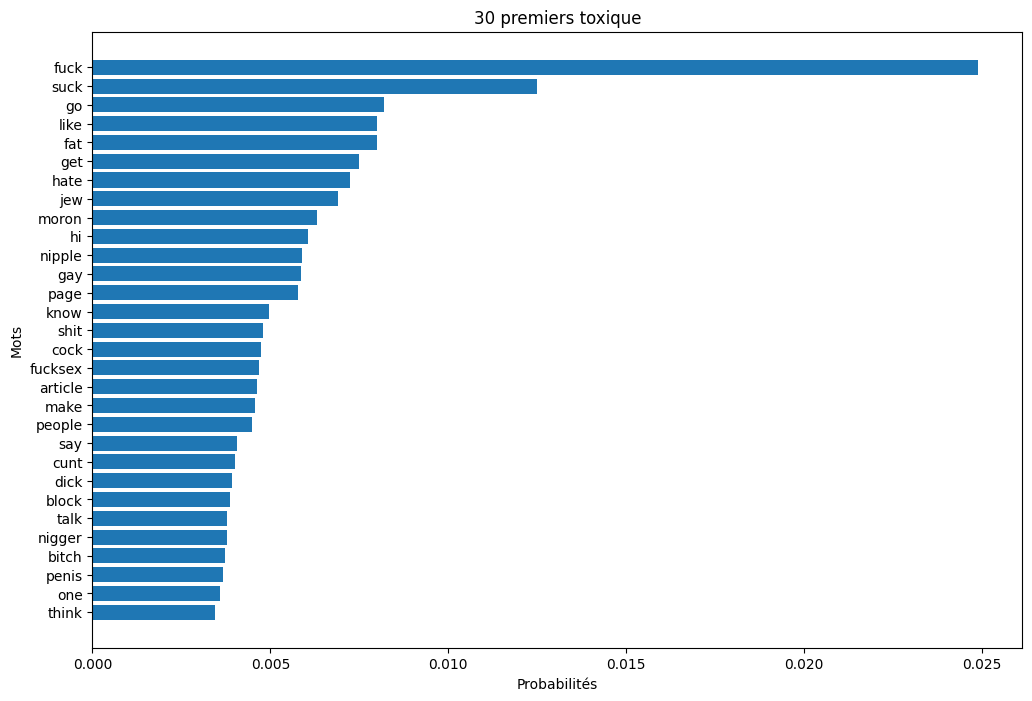
\includegraphics[width=.7\linewidth]{figures/30_first_toxic-naive_bayes.png}
    \caption{Top 30 mots toxiques}
\end{figure}

\end{document}
